\cleardoublepage

\chapter{LwM2M}

\lgf{Il est temps de voir une vrai plateforme IoT qui met en œuvre ce que nous venons d'apprendre sur CoAP et REST. Il faut installer deux programmes \Index{java}\footnote{Il s'agit d'une mise en œuvre assez ancienne, de nouvelles spécifications existent et sont quelque peu différentes, mais les concepts n'ont pas changés}~:}
\lge{It's time to see a real IoT platform that implements what we just learned about CoAP and REST. We need to install two programs \Index{java}\footnote{This is a fairly old implementation, new specifications exist and are somewhat different, but the concepts have not changed}~:}


\begin{termc}[backgroundcolor=\color{verttelecom!30}, basicstyle=\ttfamily\tiny, escapechar=@]
wget https://ci.eclipse.org/leshan/job/leshan/lastSuccessfulBuild/artifact/leshan-client-demo.jar
\end{termc}

\noindent 
\lgf{et}\lge{and}

\begin{termc}[backgroundcolor=\color{verttelecom!30}, basicstyle=\ttfamily\tiny, escapechar=@]
wget https://ci.eclipse.org/leshan/job/leshan/lastSuccessfulBuild/artifact/leshan-server-demo.jar
\end{termc}

\section{Introduction}

\lgf{\ac{LwM2M} est une architecture définie par l'\ac{OMA} à l'origine pour permettre aux opérateurs de gérer certaines ressources sur les téléphones mobiles. Mais cette architecture peut être étendu à d'autres environnement.}
\lge{\ac{LwM2M} is an architecture defined by the \ac{OMA} at the origin to allow the operators to manage certain resources on the cell phones. But this architecture can be extended to other environments.}


         \vspace{1em}

\lgf{Les spécifications sont accessibles sur le site de l'OMA\footnote{\url{https://omaspecworks.org/what-is-oma-specworks/iot/lightweight-m2m-lwm2m/}}. Nous allons utiliser une mise en œuvre en java appelé \index{Leshan}. Pas de panique nous n'allons pas programmer nous aurons juste besoin d'un navigateur Web et de \Index{Wireshark}.}
\lge{The specifications are available on the OMA site\footnote{\url{https://omaspecworks.org/what-is-oma-specworks/iot/lightweight-m2m-lwm2m/}}. We will use a java implementation called \index{Leshan}. Don't panic we are not going to program we will just need a web browser and \Index{Wireshark}.}


         \vspace{1em}

\lgf{\ac{LwM2M} comme son nom l'indique se veut léger, c'est-à-dire que les mises en œuvre ne doivent pas être trop complexes et que le trafic engendrer ne doit pas non plus être trop important. LwM2M est une plate-forme et elle va donc faire plus qu'un simple trafic REST. En particulier, l'un des rôles est de permettre aux objets de s'enregistrer et de décrire leurs caractéristiques. LmM2M va également structurer fortement les ressources en imposant des règles de nommages relativement contraintes et le format des ressources.}
\lge{As its name indicates, \ac{LwM2M} is meant to be light, meaning that the implementations should not be too complex and that the traffic generated should not be too important either. LwM2M is a platform and therefore it will do more than just REST traffic. In particular, one of the roles is to allow objects to register and describe their characteristics. LmM2M will also strongly structure the resources by imposing relatively constrained naming rules and resource format.}


\section{Architecture}

\lgf{Comme tout système qui se respecte, LwM2M fonctionne en mode client/serveur. Le serveur est la plate-forme de gestion des objets et les clients sont les objets connectés sur le réseau.}
\lge{Like any self-respecting system, LwM2M works in client/server mode. The server is the object management platform and the clients are the objects connected to the network.}


\lgf{Dans un premier temps, lancez Wireshark sur l'interface \textit{\Index{loopback}} et filtrez le trafic en le limitant au port 5683 pour UDP (celui de CoAP) en tapant \texttt{udp.port==5683}. Comme le montre la figure~\vref{fig-lwm2m-wireshark}.}
\lge{First, launch Wireshark on the interface and filter the traffic by limiting it to port 5683 for UDP (the one of CoAP) by typing \texttt{udp.port==5683}. As shown in figure~\vref{fig-lwm2m-wireshark}.}


\begin{figure}[tbp]
\centerline{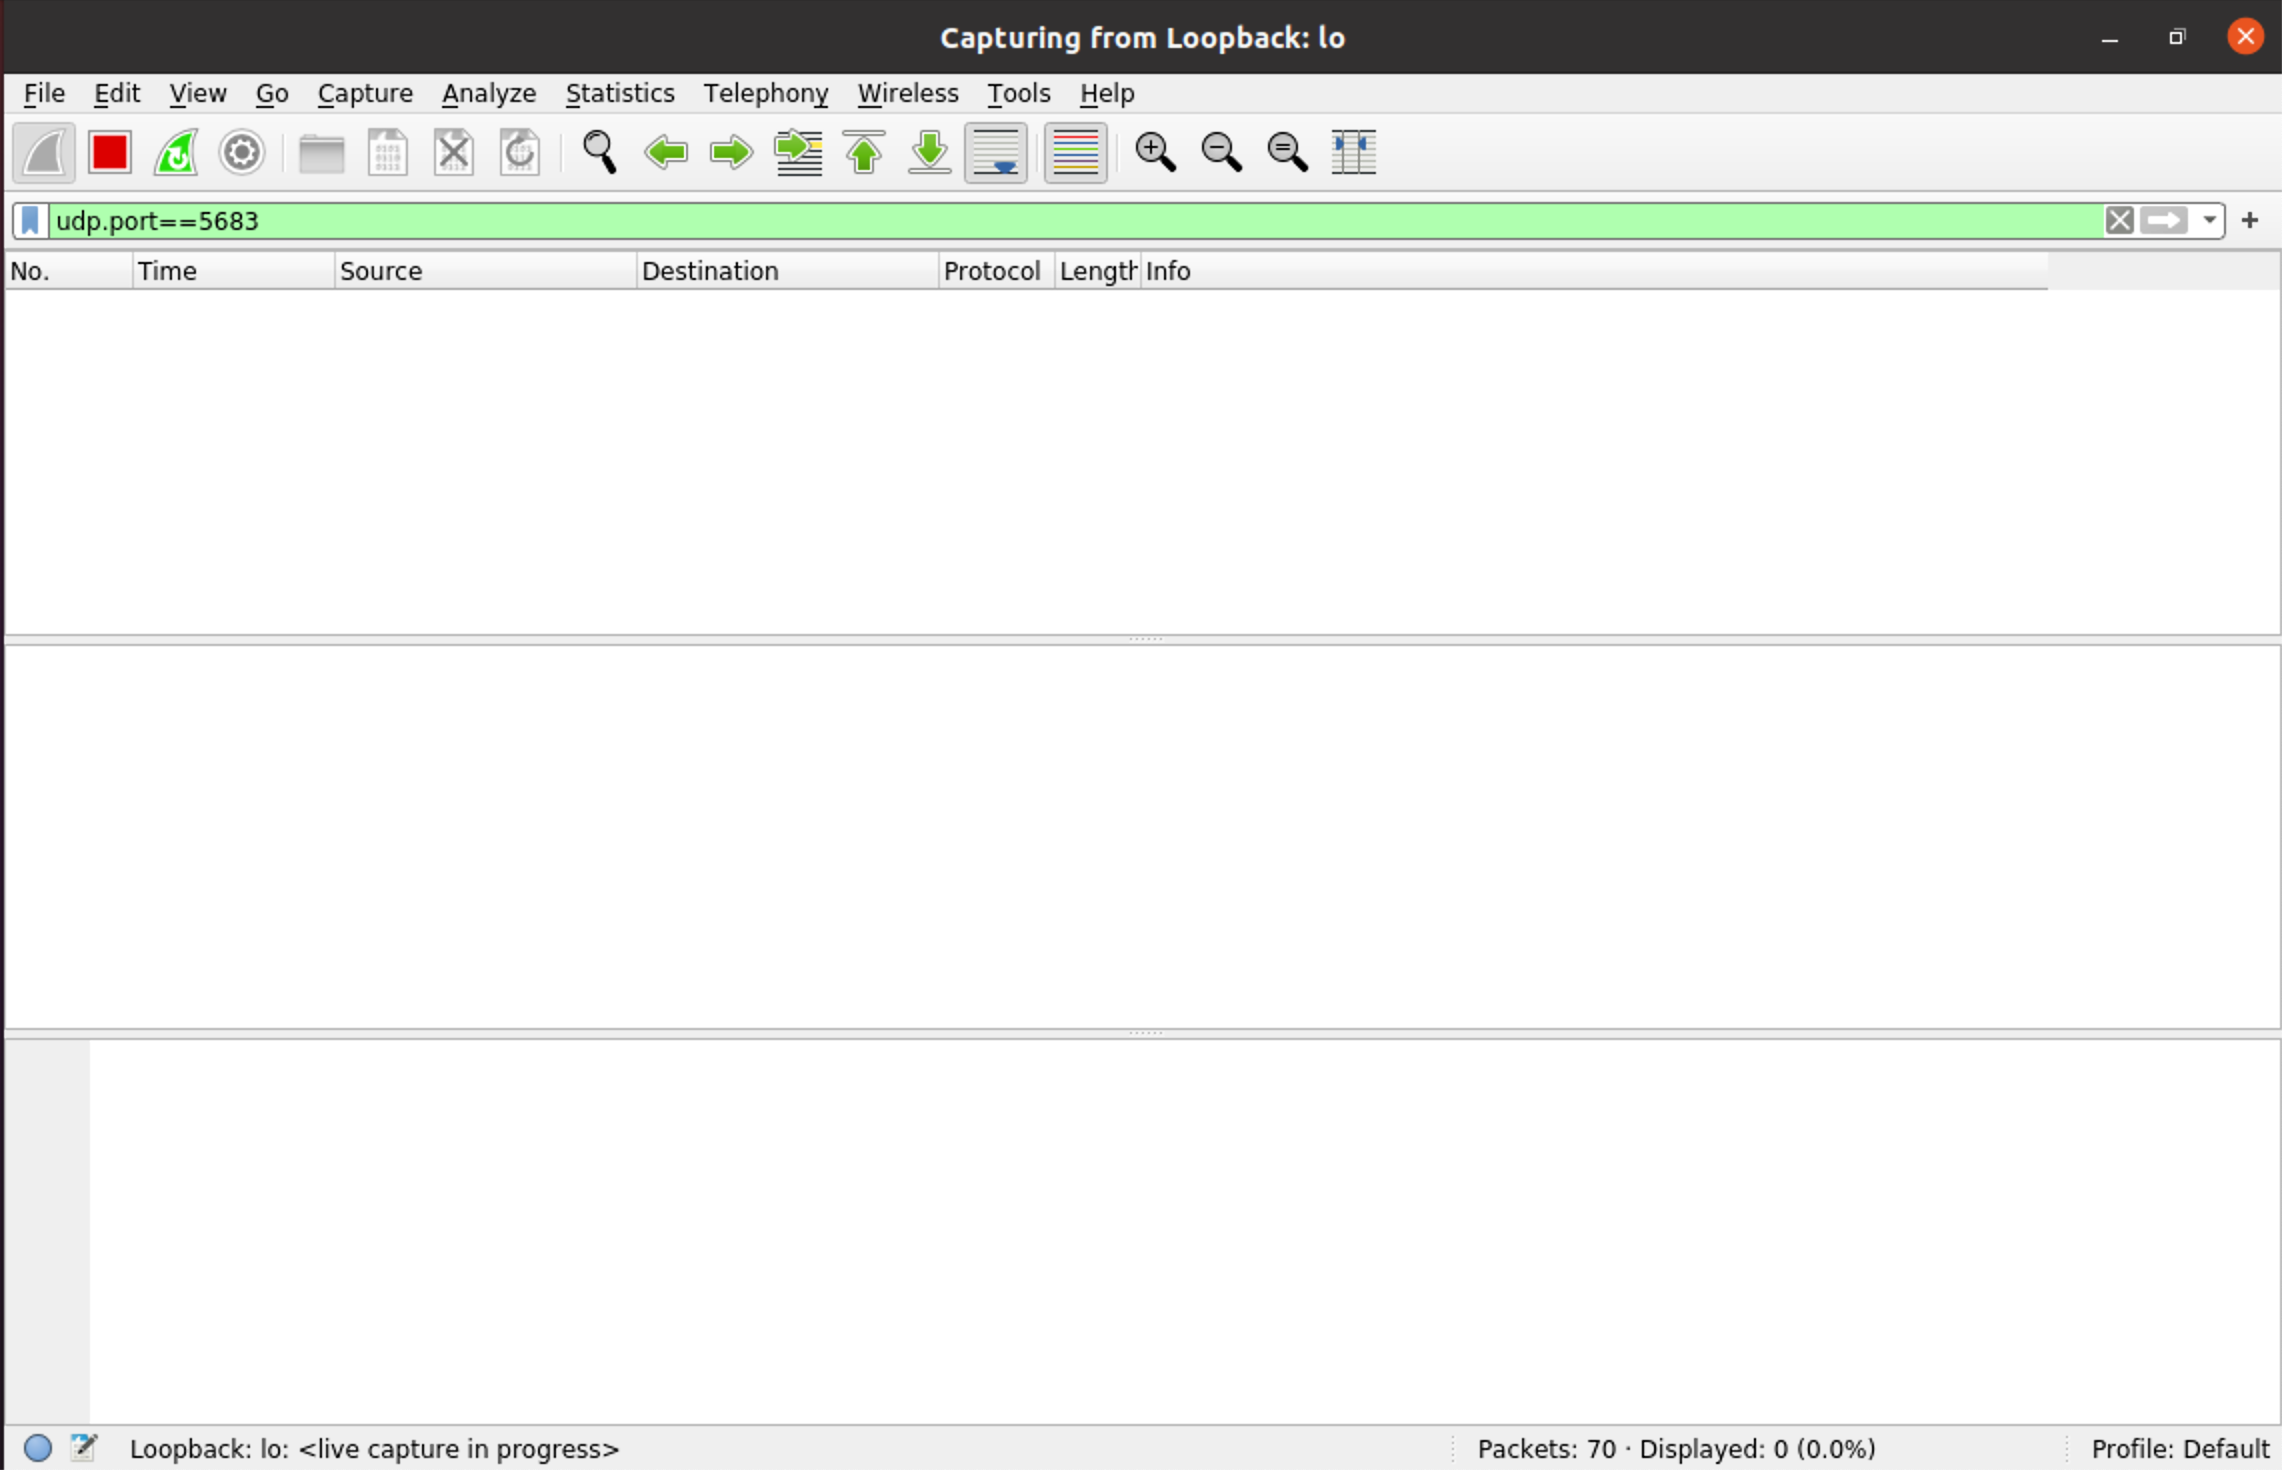
\includegraphics[width=1\columnwidth]{Pictures/lwM2M-wireshark.png}}
\lgf{\caption{Initialisation de Wireshark pour capturer le trafic CoAP}}
\lge{\caption{Initializing Wireshark to capture CoAP traffic}}

\label{fig-lwm2m-wireshark}
\end{figure}

\lgf{Nous allons maintenant lancer le serveur LwM2M, tapez\footnote{Sous Linux, tapez \texttt{apt install -y default-jre} pour installer Java.}~:}
\lge{We are now going to launch the LwM2M server, type\footnote{Under Linux, type \texttt{apt install -y default-jre} to install Java.}:}


\begin{termc}[backgroundcolor=\color{orange!40}, basicstyle=\ttfamily\small, escapechar=@] % server
> java -jar ./leshan-server-demo.jar
2020-10-22 01:34:09,365 INFO LeshanServer - LWM2M server started at
coap://0.0.0.0/0.0.0.0:5683 coaps://0.0.0.0/0.0.0.0:5684
2020-10-22 01:34:09,553 INFO LeshanServerDemo - Web server started at 
http://0.0.0.0:8080/.
\end{termc}

\lgf{Il nous indique qu'il utilise le port 5683 pour CoAP et que l'on peut superviser le serveur avec un navigateur sur le port 8080.}
\lge{It tells us that it uses port 5683 for CoAP and that we can monitor the server with a browser on port 8080.}


         \vspace{1em}

\lgf{Lancez le navigateur sur l'URI \texttt{http://127.0.0.1:8080}, la page indiqué figure~\vref{fig-lwm2m-server1} apparaît.}
\lge{Launch the browser on the URI \texttt{http://127.0.0.1:8080}, the page indicated figure~ref{fig-lwm2m-server1} appears.}


\begin{figure}[tbp]
\centerline{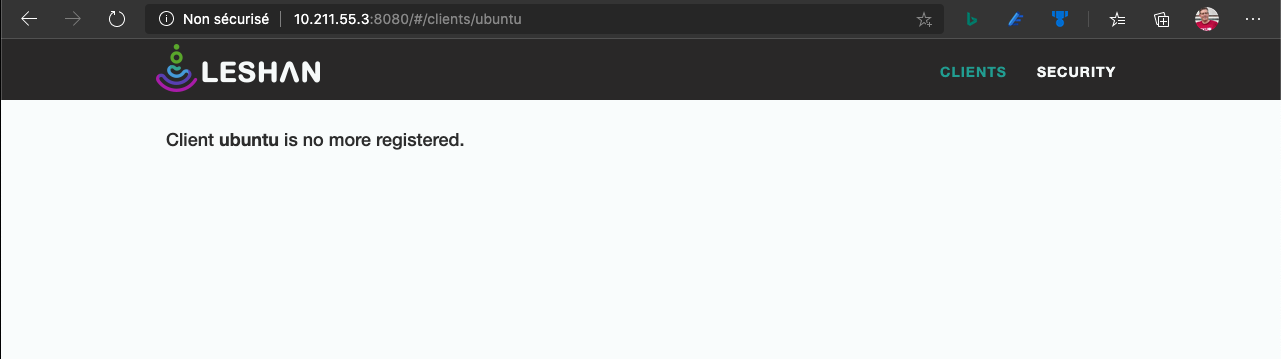
\includegraphics[width=1\columnwidth]{Pictures/lwm2m-server1.png}}
\lgf{\caption{Page d'accueil du serveur LwM2M}}
\lge{\caption{LwM2M server home page}}
\label{fig-lwm2m-server1}
\end{figure}

\lgf{Vous pouvez remarquer que l'ouverture du serveur LwM2M n'a provoqué aucun trafic CoAP sur l'analyseur réseau.}
\lge{You may notice that opening the LwM2M server did not cause any CoAP traffic on the network analyzer.}


         \vspace{1em}

\lgf{Lancez maintenant dans une autre fenêtre, le client LwM2M:}
\lge{Now launch the LwM2M client in another window:}

\begin{termc}[backgroundcolor=\color{purple!30}, basicstyle=\ttfamily\small, escapechar=@] % client
> java -jar ./leshan-client-demo.jar
2020-10-22 01:49:51,063 INFO LeshanClientDemo - Commands available :

  - create <objectId> : to enable a new object.
  - delete <objectId> : to disable a new object.
  - update : to trigger a registration update.
  - w : to move to North.
  - a : to move to East.
  - s : to move to South.
  - d : to move to West.

2020-10-22 01:49:51,064 INFO LeshanClient - Starting Leshan client ...
2020-10-22 01:49:51,158 INFO CaliforniumEndpointsManager - New 
endpoint created for server coap://localhost:5683 at 
coap://0.0.0.0:48274
2020-10-22 01:49:51,159 INFO LeshanClient - Leshan client
[endpoint:ubuntu] started.
2020-10-22 01:49:51,160 INFO DefaultRegistrationEngine - Trying to 
register to coap://localhost:5683 ...
2020-10-22 01:49:51,252 INFO DefaultRegistrationEngine - Registered 
with location '/rd/BOr5Pg7yW8'.
2020-10-22 01:49:51,252 INFO DefaultRegistrationEngine - Next 
registration update to coap://localhost:5683 in 53s...
\end{termc}

\lgf{\section{Enregistrement d'un Objet}}
\lge{\section{Registration of an Object}}

\lgf{Comme nous utilisons une adresse \textit{loopback}, il est un peu plus difficile de repérer dans la trafic Wireshark récupéré (cf. figure~\vref{fig-lwm2m-bootstrap}) qui est le client et qui est le serveur. Mais comme Le serveur attend sur le port 5683, en regarda,t de plus près un paquet, on peut déterminé s'il a été émis par le client ou le serveur.}
\lge{Since we are using an address, it is a bit more difficult to identify in the recovered Wireshark traffic (see figure~\vref{fig-lwm2m-bootstrap}) who is the client and who is the server. But since the server is waiting on port 5683, by looking more closely at a packet, we can determine whether it was sent by the client or the server.}


\begin{figure}[tbp]
\centerline{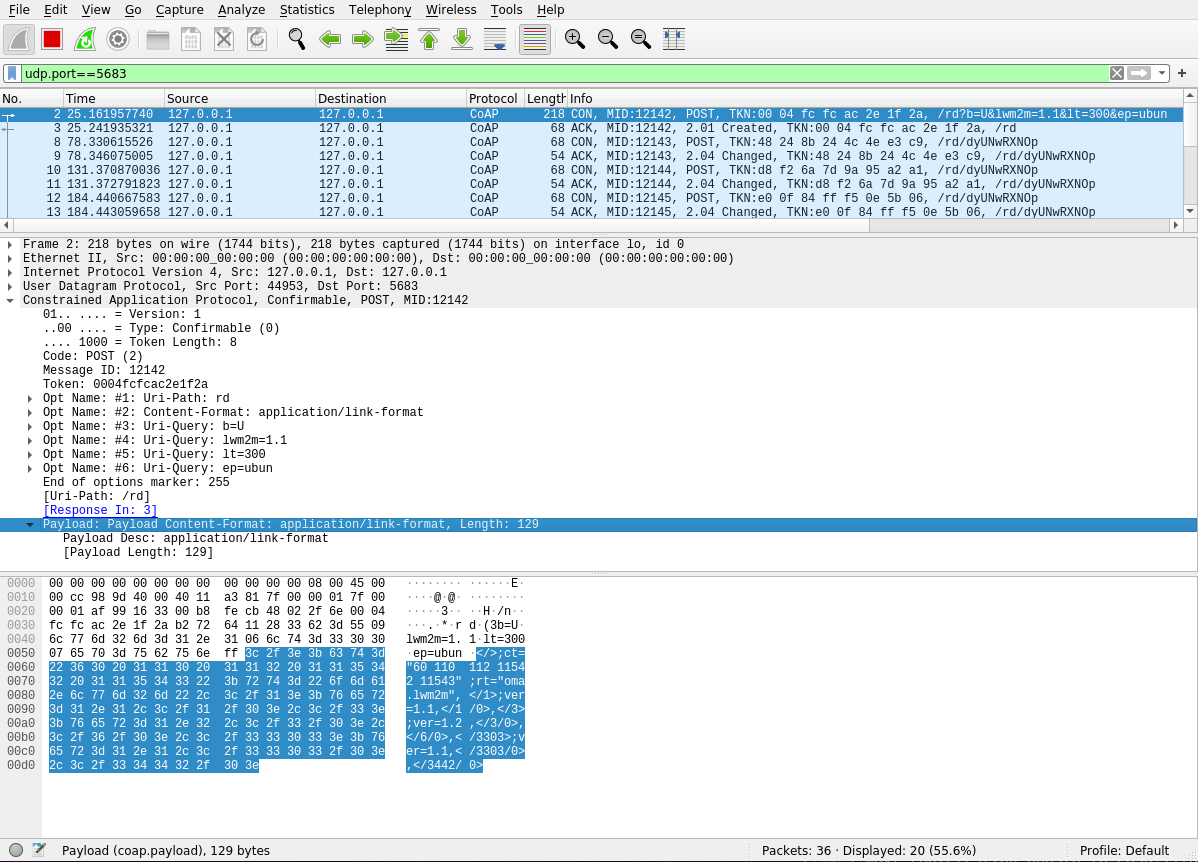
\includegraphics[width=.9\columnwidth]{Pictures/lwm2m-bootstrap.png}}
\lgf{\caption{Premières captures LwM2M}}
\lge{\caption{First LwM2M captures}}
\label{fig-lwm2m-bootstrap}
\end{figure}

\lgf{\subsection{Analyse de l'en-tête CoAP}}
\lge{\subsection{Analysis of the CoAP header}}

\lgf{On peut voir sur la trace, que le client contacte le serveur pour lui indiquer ses propriétés.}
\lge{We can see on the trace, that the client contacts the server to indicate its properties.}


\Question{\lgf{Méthode}\lge{Method}}
{
\lgf{Quelle est la nature de la requête émise par le client~:}
\lge{What is the nature of the request issued by the client~:}

\begin{itemize}[label=$\circ$]
   \item \Wrong{GET}
   \item \Correct{POST}
   \item \Wrong{PUT}
   \item \Wrong{DELETE}
\end{itemize}}
{
\lgf{Le client LwM2M agit comme un client REST et envoie cette requête POST~:\\}
\lge{The LwM2M client acts as a REST client and sends this POST request :\\}
\noindent\texttt{
Constrained Application Protocol, Confirmable, POST, MID:12142\\
    01.. .... = Version: 1\\
    ..00 .... = Type: Confirmable (0)\\
    .... 1000 = Token Length: 8\\
    Code: POST (2)\\
    Message ID: 12142\\
}
}

\Question{URI}
{
\lgf{Quelle est le chemin de l'URI~:}
\lge{What is the path of the URI~:}

\begin{itemize}[label=$\circ$]
   \item \Wrong{\lgf{vide}\lge{empty}}
   \item \Correct{/rd}
   \item \Wrong{/lwm2m}
\end{itemize}}
{
\lgf{Le chemin d'URI est composé s'un seul élément~:\\}
\lge{The URI path is composed of a single element:\\}
\noindent\texttt{
    Opt Name: #1: \Index{Uri-Path}: rd\\
}

}

\Question{Content}
{
\lgf{Quelle est le format du contenu (content-format)~:}
\lge{What is the format of the content (content-format)~:}
\begin{itemize}[label=$\circ$]
   \item \Wrong{text}
   \item \Wrong{XML}
   \item \Wrong{JSON}
   \item \Correct{link-format}
   \item \Wrong{CBOR}
\end{itemize}}
{
\lgf{Après le chemin d'URI on trouve l'option Content-Format qui contient la valeur 40 soit \Index{link-format}~:\\}
\lge{After the URI path we find the Content-Format option which contains the value 40 or \Index{link-format}:\\}
\noindent\texttt{
    Opt Name: #2: \Index{Content-Format}: application/link-format
}
}

\Question{\lgf{Période}\lge{Period}}
{
\lgf{A quelle periode voyez vous d'afficher des messages CoAP ?}
\lge{What is the period in which you see CoAP messages?}
}
{
\lgf{La figure~\vref{fig-lwm2m-bootstrap} montre plusieurs échanges. Le premier à 25.16 secondes est un POST sur /rd. Le second à 78.33 secondes un POST sur /rd/dyUNwRXNOp. Le troisième à 131.37 secondes est identique et les suivants sont identiques. La période d'envoi est de 53 secondes.}
\lge{Figure~\vref{fig-lwm2m-bootstrap} shows several exchanges. The first one at 25.16 seconds is a POST to /rd. The second at 78.33 seconds is a POST to /rd/dyUNwRXNOp. The third at 131.37 seconds is identical and the following ones are identical. The sending period is 53 seconds.}
}

\lgf{Pour décoder l'Uri-Query de la requête CoAP il faut d'aider du document \href{http://www.openmobilealliance.org/release/LightweightM2M/V1_1_1-20190617-A/OMA-TS-LightweightM2M_Core-V1_1_1-20190617-A.pdf}{LwM2M Core Specification}\footnote{\url{http://www.openmobilealliance.org/release/LightweightM2M/V1_1_1-20190617-A/OMA-TS-LightweightM2M_Core-V1_1_1-20190617-A.pdf}} et de son tableau 6.2.1 page 40. }
\lge{To decode the Uri-Query of the CoAP request it is necessary to help the document \href{http://www.openmobilealliance.org/release/LightweightM2M/V1_1_1-20190617-A/OMA-TS-LightweightM2M_Core-V1_1_1-20190617-A.pdf}{LwM2M Core Specification}\footnote{\url{http://www.openmobilealliance.org/release/LightweightM2M/V1_1_1-20190617-A/OMA-TS-LightweightM2M_Core-V1_1_1-20190617-A.pdf}} and its table 6.2.1 page 40. }

\Question{b=U}
{
\lgf{Que signifie b=U ?}
\lge{What does b=U mean?}

\begin{itemize}[label=$\circ$]
   \item \Wrong{
    \lgf{Les données seront émises avec les unités (Units)}
    \lge{The data will be sent with the units}
    }
   \item \Wrong{
    \lgf{Le référenciel des unités est la représentation Universelle}
    \lge{The reference of the units is the Universal representation}
    }
   \item \Correct{
    \lgf{Le protocole sous-jacent est en mode datagramme (UDP)}
    \lge{The underlying protocol is in datagram mode (UDP)}
    }
   \item \Wrong{
    \lgf{Le client n'est pas référencé (Unreferenced)}
    \lge{The client is not referenced (Unreferenced)}
    }
\end{itemize}
}
{
\lgf{Ce paramètre désigne le \texitit{binding}, U indique que CoAP sera transporté sur UDP. Le standard propose également d'autres modes, comme~:}
\lge{This parameter designates the \texitit{binding}, U indicates that CoAP will be transported over UDP. The standard also offers other modes, such as:}
\begin{itemize}
    \item  
        \lgf{T : TCP. CoAP prévoit également un mode de fonctionnement sur \Index{TCP} (\rfc{8323}). Le mode permet par exemple de traverser des réseaux qui restreignent l'usage d'~\Index{UDP} pour de soit disant raisons de sécurité;}
        \lge{T : TCP. CoAP also provides a mode of operation over \Index{TCP} (\rfc{8323}). The mode allows for example to cross networks which restrict the use of ~Index{UDP} for so-called security reasons;}
    \item 
        \lgf{S : SMS. LwM2M est défini par l'\acl{OMA}, il est logique d'inclure ce moyen de communication pour gérer un équipement connecté au réseau cellulaire~;}
        \lge{S: SMS. LwM2M is defined by the \acl{OMA}, it is logical to include this means of communication to manage an equipment connected to the cellular network~;}
    \item 
        \lgf{N : \Index{NON-IP}. Dans ce mode, les messages CoAP sont directement envoyés sur le niveau 2. Il est également connu sous le terme de \ac{NIDD} dans les réseaux 4G.}
        \lge{N : \Index{NON-IP}. In this mode, CoAP messages are sent directly on level 2. It is also known as \ac{NIDD} in 4G networks.}
    \item 
        \lgf{Nous nous basons sur la version 1.1 du standard, la révision 1.2 de LwM2M intègre également de LoRaWAN, MQTT (M), HTTP (H),...}
        \lge{We are based on version 1.1 of the standard, revision 1.2 of LwM2M also integrates LoRaWAN, MQTT (M), HTTP (H),...}
\end{itemize}
}


\Question{lwm2m=1.1}
{
\lgf{Que signifie lwm2m=1.1 ? Il s'agit...}
\lge{What does lwm2m=1.1 mean? It is a question of...}

\begin{itemize}[label=$\circ$]
   \item \Correct{
    \lgf{de la version lwm2m du client}
    \lge{the lwm2m client version}
    }
   \item \Wrong{
    \lgf{de la taille mémoire de l'implémentation (1.1 ko)}
    \lge{the memory size of the implementation (1.1 kb)}
    }
   \item \Wrong{
    \lgf{de la version lwm2m du serveur}
    \lge{the lwm2m server version}
    }
\end{itemize}
}
{
\lgf{Il s'agit de la version du client. }
\lge{This is the client's version. }
}

\Question{lt=300}{
\lgf{Que signifie lt=300 ?}
\lge{What does lt=300 mean?}

\begin{itemize}[label=$\circ$]
   \item \Wrong{
    \lgf{C'est le nombre maximal d'objets (less than 300)}
    \lge{This is the maximum number of objects (less than 300)}
    }
   \item \Wrong{
    \lgf{C'est la taille maximale d'un échange (300 octets)}
    \lge{This is the maximum size of an exchange (300 bytes)}
    }
   \item \Correct{
    \lgf{C'est la durée de vie de l'enregistrement d'un objet (lifetime)}
    \lge{This is the lifetime of an object's registration}
    }
\end{itemize}
}
{
\lgf{C'est la durée de vie d'une valeur, si elle n'est pas rafraîchie avant ce délais par le client, elle disparaîtra du serveur.}
\lge{This is the lifetime of a value, if it is not refreshed before this time by the client, it will disappear from the server.}
}

\lgf{\subsection{Analyse du contenu du POST}}
\lge{\subsection{POST Content Analysis}}


\lgf{Revenons au contenu du message de la requête POST émise initialement par le client. Que veut dire \Index{link-format}~? Nous n'avons pas encore vu ce format. Heureusement, l'\ac{IANA} est notre ami et en allant chercher à quoi correspond cette valeur, sur cette page \footnote{\url{https://www.iana.org/assignments/core-parameters/core-parameters.xhtml\#content-formats}}, on trouve que le \rfc{6690} définit ce contenu.}
\lge{Let's go back to the message content of the POST request initially sent by the client. What does \Index{link-format}~ mean? We haven't seen this format yet. Fortunately, the \ac{IANA} is our friend and by going to look for what this value corresponds to, on this page \footnote{\url{https://www.iana.org/assignments/core-parameters/core-parameters.xhtml\#content-formats}}, we find that the \rfc{6690} defines this content.}


\lgf{Il utilise un format particulier qui est utilisé initialement par le Web pour définir des relations entre pages initialement définit dans le \rfc{5988}. Il est important de remarquer, et après la lecture devient plus claire, que les URI sont notées entre \texttt{<>}. Ensuite, on trouve des attributs liés à cet URI séparés par des points-virgules. Les virgules séparent les définitions.}
\lge{It uses a particular format which is used initially by the Web to define relations between pages initially defined in the \rfc{5988}. It is important to notice, and after the reading becomes clearer, that the URI are noted between \texttt{<>}. Then, we find attributes linked to this URI separated by semicolons. The commas separate the definitions.}

\lgf{En suivant ces règles de notation, les données émises par le client peuvent être formatés de la manière suivante :}
\lge{En suivant ces règles de notation, les données émises par le client peuvent être formatés de la manière suivante :}


\begin{termc}[backgroundcolor=\color{purple!30}, basicstyle=\ttfamily\small, escapechar=@] % client
</>;ct="60 110 112 11542 11543";rt="oma.lwm2m",
</1>;ver=1.1,
</1/0>,
</3>;ver=1.2,
</3/0>,
</6/0>,
</3303>;ver=1.1,
</3303/0>,
</3442/0>
\end{termc}

\lgf{Le client utilise ce format pour décrire les 9 ressources qu'il possède et qui sont identifiées par ces 9 chemins d'URI. Le nommage des ressources peut paraître étrange ; nous verrons par la suite à quoi il correspond~:}
\lge{The client uses this format to describe the 9 resources it owns, which are identified by these 9 URI paths. The naming of the resources may seem strange; we will see later what it corresponds to:}


\begin{itemize}
    \item 
        \lgf{La première ligne concerne la racine \texttt{</>} pour laquelle deux attributs sont associés, il seront donc applicable à l'ensemble des éléments. }
        \lgf{La première ligne concerne la racine \texttt{</>} pour laquelle deux attributs sont associés, il seront donc applicable à l'ensemble des éléments. }
    \begin{itemize}
        \item  
            \lgf{Le premier \texttt{\Index{ct}}\footnote{Voir \rfc{7252} chapitre 7.2.} définit les formats des représentations possible des objets. La partie entre guillemets fait références aux valeurs de Content-format de CoAP listé tableau~\vref{tab-CoAP-MIME}. On y retrouve respectivement les types CBOR, SenML et pour les deux derniers un format orienté TLV propre à LwM2M.}
            \lge{The first \texttt{\Index{ct}}\footnote{See \rfc{7252} chapter 7.2.} defines the formats of the possible representations of the objects. The part between quotation marks refers to the Content-format values of CoAP listed in table~\vref{tab-CoAP-MIME}. We find there respectively the CBOR, SenML types and for the last two a TLV oriented format specific to LwM2M.}
        \item 
            \lgf{Le second \texttt{\Index{rt}}\footnote{Voir \rfc{6690} chapitre 3.1.} indique le type de ressource (\textit{resource-type}), c'est-à-dire indique comment elles seront représentées. Ici, cela indique que les ressources suivront les spécifications \ac{LwM2M} de l'\ac{OMA}.}
            \lge{The second \texttt{\Index{rt}}\footnote{Voir \rfc{6690} chapter 3.1.}  indicates the type of resource (\textit{resource-type}), i.e. how they will be represented. Here, it indicates that the resources will follow the \ac{LwM2M} specifications of the \ac{OMA}.}
    \end{itemize}
    \item 
        \lgf{Les lignes suivantes décrivent, toujours de manière hiérarchique, les chemins d'URI et les attributs associés. L'attribut \texttt{\Index{ver}} indique la version du standard utilisée pour définir la ressource.}
        \lge{The following lines describe, again in a hierarchical manner, the URI paths and associated attributes. The attribute \texttt{Index{ver}} indicates the version of the standard used to define the resource.}
 
\end{itemize}


\Question{rt}{
\lgf{À quoi sert l'attribut rt ?}
\lge{What is the purpose of the rt attribute?}

\begin{itemize}[label=$\circ$]
   \item \Correct{
    \lgf{à donner la sémantique (i.e. comment interpréter) de la ressource.}
    \lge{to give the semantics (i.e. how to interpret) of the resource.}
    }
   \item \Wrong{
    \lgf{à indiquer la taille de la ressource en faisant référence à lwm2m.}
    \lge{to indicate the size of the resource with reference to lwm2m.}
    }
   \item \Wrong{
    \lgf{à indiquer la version de lwm2m utilisée.}
    \lge{to indicate the version of lwm2m used.}
    }
   \item \Wrong{
    \lgf{à aider à déboguer les échanges.}
    \lge{to help debug the exchanges.}
    }
\end{itemize}
 }{
 \lgf{Quand le serveur reçoit le POST du client, il est capable d'associer une représentation au chemin d'URI décrit. Le client et le serveur doivent avoir cette connaissance à priori.}
 \lge{When the server receives the POST from the client, it is able to associate a representation with the described URI path. Both the client and the server must have this knowledge a priori.}
 }

\lgf{\subsection{Définition des ressources}}

\lgf{LwM2M représente les ressources d'une manière assez originale pour être à la fois compact, universel (ce qui est quelquefois oxymorique) et flexible. Pour ce faire, tout est désigné par des chiffres.  Le chapitre 7 page 63 du document. principal\footnote{\url{http://www.openmobilealliance.org/release/LightweightM2M/V1_1_1-20190617-A/OMA-TS-LightweightM2M_Core-V1_1_1-20190617-A.pdf}} contient le schéma figure~\vref{fig-lwm2m-objects}  illustrant cette hiérarchie~:  }
\lge{LwM2M represents resources in a way that is original enough to be both compact, universal (which is sometimes oxymoronic) and flexible. To do this, everything is designated by numbers.  Chapter 7 page 63 of the document. principalfootnote{\url{http://www.openmobilealliance.org/release/LightweightM2M/V1_1_1-20190617-A/OMA-TS-LightweightM2M_Core-V1_1_1-20190617-A.pdf}} contains the figure~\vref{fig-lwm2m-objects} diagram illustrating this hierarchy~:  }


\begin{figure}[tbp]
\centerline{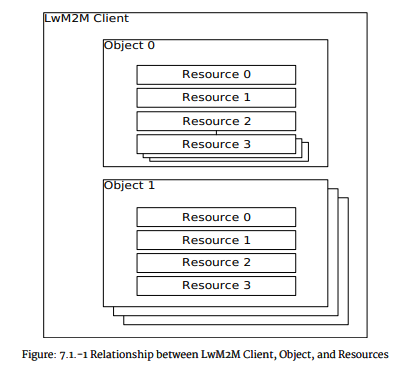
\includegraphics[width=.6\columnwidth]{Pictures/lwm2m-objects.png}}
\caption{Hierarchie de nommage}
\label{fig-lwm2m-objects}
\end{figure}

\begin{itemize}
\item 
    \lgf{Un Objet physique (ie notre client) contient une liste d'objets numériques\footnote{LwM2M appelle cette information \textit{object} ce qui rend en français la définition ambiguë puisque Objet est aussi la traduction de \textit{thing}} identifié par un numéro. Ce numéro est attribué par l'OMA. Par exemple, un capteur de température aura la valeur \textit{\texttt{3303}}. Une liste des valeurs déjà attribuées peut être trouvée à cette \href{http://www.openmobilealliance.org/wp/OMNA/LwM2M/LwM2MRegistry.html#resources}{adresse}\footnote{\url{http://www.openmobilealliance.org/wp/OMNA/LwM2M/LwM2MRegistry.html#resources}}. }
    \lge{A physical Object (i.e. our client) contains a list of numerical objects. LwM2M calls this information \textit{object} which makes the definition ambiguous since Objet is also the translation of \textit{thing} identified by a number. This number is assigned by the OMA. For example, a temperature sensor will have the value \textit{\Òtexttt{3303}}. A list of previously assigned values can be found at this \href{http://www.openmobilealliance.org/wp/OMNA/LwM2M/LwM2MRegistry.html#resources}{address}\footnote{\url{http://www.openmobilealliance.org/wp/OMNA/LwM2M/LwM2MRegistry.html#resources}}. }
    
\item 
    \lgf{Un client peut évidemment posséder plusieurs instance d'un objet numérique, par exemple, une station météo pourrait avoir un capteurs de température intérieur et extérieur. Le deuxième chiffre du chemin de l'URI indique cette instance. S'il n'y en a qu'un, il prend la valeur \textit{\textttt{0}}.}
    \lge{Un client peut évidemment posséder plusieurs instance d'un objet numérique, par exemple, une station météo pourrait avoir un capteurs de température intérieur et extérieur. Le deuxième chiffre du chemin de l'URI indique cette instance. S'il n'y en a qu'un, il prend la valeur \textit{\textttt{0}}.}
    
\item 
    \lgf{Finalement, l'objet peut être complexe et contenir plusieurs informations appelée ressouces. En cliquant sur le chiffre \textit{\textttt{3303}} dans la page web précédente, on obtient la description de l'objet. On peut voir que :}
    \lge{Finally, the object can be complex and contain several information called resources. By clicking on the number \textit{textttt{3303}} in the previous web page, we obtain the description of the object. We can see that :}
    
\begin{itemize}
\item \textit{\textttt{5700}} 
    \lgf{représente la valeur mesurée par le capteur}
    \lge{represents the value measured by the sensor}
\item \textit{\textttt{5601}} 
    \lgf{la valeur minimale}
    \lge{the minimum value}
\item \textit{\textttt{5602}} 
    \lgf{la valeur maximale}
    \lge{the maximum value}
\item \textit{\textttt{5701}} 
    \lgf{indique les unités }
    \lge{indicates the units }
\item \textit{\textttt{5605}} 
    \lgf{permet de remettre à zéro le calcul des minima et maxima}
    \lge{allows you to reset the calculation of minimum and maximum values}
\end{itemize}
    \lgf{Ces valeurs peuvent se retrouver dans plusieurs objets numériques.}
    \lge{These values can be found in several numerical objects.}
    
\item 
    \lgf{la version 1.2 du standard introduit également la possibilité d'avoir plusieurs instances d'une ressource.}
    \lge{version 1.2 of the standard also introduces the possibility to have several instances of a resource.}
\end{itemize}

\lgf{\subsubsection{Valeurs associées aux objets numériques}}

\lgf{Les objets numériques peuvent être définit par LwM2M, ils concernent ceux dédié à la gestion du protocole. Par exemple, l'objet numérique~:}
\lge{Digital objects can be defined by LwM2M, they concern those dedicated to the management of the protocol. For example, the digital object~:}


\begin{itemize}
    \item  
        \lgf{\textit{\textttt{0}} définit l'environnement de sécurité du client. Il contient l'adresse du serveur, les clés de chiffrement,\ldots}
        \lge{\textit{\textttt{0}} defines the security environment of the client. It contains the server address, the encryption keys,\ldots}
        
    \item 
        \lgf{\textit{\textttt{1}} définit les paramètres pour la communication avec le serveur, comme par exemple la durée de vie de l'information en seconde,\ldots}
        \lge{\textit{\textttt{1}} defines the parameters for the communication with the server, such as the lifetime of the information in seconds,\ldots}
        
    \item 
        \lgf{\textit{\textttt{3}} describes the characteristics of the equipment as its software version,\ldots}
        \lge{\textit{\textttt{3}} describes the characteristics of the equipment such as its software version,\ldots}
        
    \item \ldots
\end{itemize}

         \vspace{1em}


\lgf{Les valeurs comprises entre 2~048 et 10~240 sont définies par des organismes de standardisation partenaire de l'\ac{OMA},  comme par exemple~:}
\lge{The values between 2~048 and 10~240 are defined by partner standardization organizations of \ac{OMA}, such as~:}

\begin{itemize}
    \item 
        \lgf{l'\acro{IPSO} Alliance qui va définir des objets numériques types, comme un capteur de température ayant pour référence \textit{\textttt{3303}},}
        \lge{the \acro{IPSO} Alliance which will define typical digital objects, such as a temperature sensor with reference \textit{textttt{3303}},}
        
    \item 
        \lgf{la \acro{GSMA} qui définit les objets pour la gestion des téléphones cellulaire,}
        \lgf{the \acro{GSMA} which defines the objects for the management of cell phones,}
        
    \item \ldots
\end{itemize}

\lgf{Les valeurs supérieures sont réservées aux industriels qui peuvent enregistrer leurs propres spécifications.}
\lge{Higher values are reserved for manufacturers who can register their own specifications.}

\lgf{\subsubsection{Valeurs associées aux ressources}}
\lge{\subsubsection{Values associated with resources}}

\lgf{La figure~\vref{fig-lwm2m-3303}, copiée du site Web de l'\ac{OMA}, donne un exemple de définition d'un objet numérique. A l'objet 3303 sont associés un certain nombre de ressources, générique que l'on peut aussi trouver dans d'autres objets numérique. Ainsi~:}
\lge{The figure~\vref{fig-lwm2m-3303}, copied from the \ac{OMA} website, gives an example of the definition of a digital object. To the object 3303 are associated a certain number of resources, generic that can also be found in other digital objects. Thus~:}


\begin{figure}[tbp]
\centerline{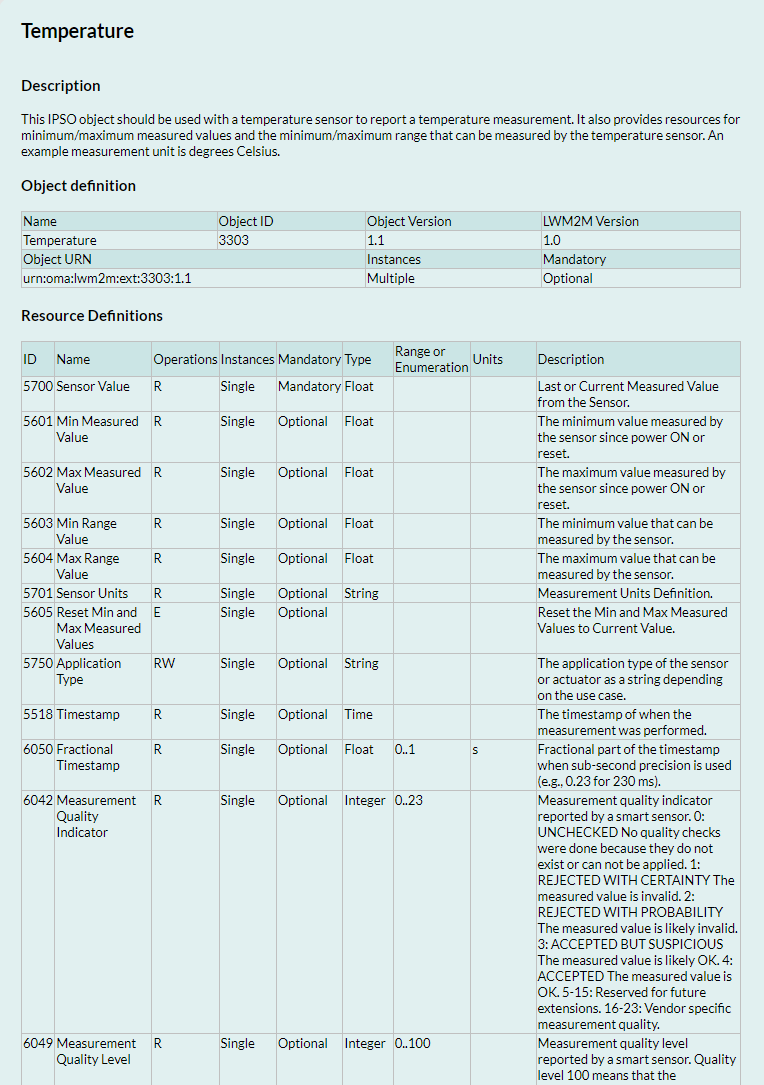
\includegraphics[width=1\columnwidth]{Pictures/lwm2m-3303.png}}
\lgf{\caption{Définition de l'objet numérique 3303 pour la température}}
\lge{\caption{Definition of the numerical object 3303 for the temperature}}
\label{fig-lwm2m-3303}
\end{figure}

\begin{itemize}
    \item \textit{\textttt{5700}} 
        \lgf{frefers to the measured value represented as a floating number. This number can only be read (\texttt{R})}
        \lge{fait référence à la valeur mesurée représenté comme un nombre flottant. Ce nombre ne peut que être lu (\texttt{R})}
        
    \item \textit{\textttt{5700}} 
        \lgf{est une chaîne de caractère qui précise l'unité de mesure.}
        \lge{is a string that specifies the unit of measurement.}
        
    \item \textit{\textttt{5601}} 
        \lgf{et}\lge{and} 
        \textit{\textttt{5602}} 
        \lgf{conservent les valeurs minimales et maximales. Elle peuvent être remise à zéro via la ressource \textit{\textttt{5605}} qui conduit à une exécution d'un programme (\texttt{E}).}
        \lge{keep the minimum and maximum values. They can be reset via the resource \textit{\textttt{5605}} which leads to a program execution (\texttt{E}).}
        
    \item  \textit{\textttt{5603}} 
        \lgf{et}\lge{and}  \textit{\textttt{5604}} 
        \lgf{correspondent à la plage d'utilisation du capteur et ne peuvent pas être modifiées.}
        \lge{are within the operating range of the sensor and cannot be changed.}
\end{itemize}


         \vspace{1em}
         
\lgf{Ainsi \textit{\texttt{3303/3/5601}} représente la valeur minimale (\textit{\textttt{5601}}) du quatrième capteur (\textit{\textttt{3}} car on commence à 0) de l'objet numérique température (\textit{\textttt{3303}}).}
\lge{Thus \textit{\textttt{3303/3/5601}} represents the minimum value (\textit{\textttt{5601}}) of the fourth sensor (\textit{\textttt{3}} because we start at 0) of the numerical object temperature (\textit{\textttt{3303}}).}


\lgf{Par rapport à \Index{Modbus}, où l'on devait télécharger la documentation de l'Objet (cf tableau~\vref{tab-meter-IR}), LwM2M offre une manière standard de décrire l'information produite ou consommée par un Objet. De plus, la définition de l'objet numérique, en plus d'être visualisable sous forme de tableau sur le site web, existe aussi en \Index{XML} pour être traitée informatiquement et permettre l'interopérabilité.}
\lge{Compared to \Index{Modbus}, where one had to download the documentation of the Object (cf table~\vref{tab-meter-IR}), LwM2M offers a standard way to describe the information produced or consumed by an Object. Moreover, the definition of the digital object, in addition to being visualized in the form of table on the Web site, also exists in index{XML} to be treated informatically and to allow interoperability.}


\begin{termc}[backgroundcolor=\color{blue!10}, basicstyle=\ttfamily\tiny, escapechar=@, language=xml] % client
<?xml version="1.0" encoding="UTF-8"?>

<!-- BSD-3 Clause License ... -->

<LWM2M  xmlns:xsi="http://www.w3.org/2001/XMLSchema-instance" xsi:noNamespaceSchemaLocation=
"http://openmobilealliance.org/tech/profiles/LWM2M.xsd">
	<Object ObjectType="MODefinition">
		<Name>Temperature</Name>
		<Description1>
		    This IPSO object should be used with a temperature sensor to report a temperature
		    measurement.  It also provides resources for minimum/maximum measured values and the
		    minimum/maximum range that can be measured 
		    by the temperature sensor. An example measurement unit is degrees Celsius.
		</Description1>
		<ObjectID>3303</ObjectID>
		<ObjectURN>urn:oma:lwm2m:ext:3303:1.1</ObjectURN>
		<LWM2MVersion>1.0</LWM2MVersion>
		<ObjectVersion>1.1</ObjectVersion>
		<MultipleInstances>Multiple</MultipleInstances>
		<Mandatory>Optional</Mandatory>
		<Resources>
			<Item ID="5700">
				<Name>Sensor Value</Name>
				<Operations>R</Operations>
				<MultipleInstances>Single</MultipleInstances>
				<Mandatory>Mandatory</Mandatory>
				<Type>Float</Type>
				<RangeEnumeration></RangeEnumeration>
				<Units></Units>
				<Description>Last or Current Measured Value from the Sensor.</Description>
			</Item>
			<Item ID="5601">
				<Name>Min Measured Value</Name>
				<Operations>R</Operations>
				<MultipleInstances>Single</MultipleInstances>
				<Mandatory>Optional</Mandatory>
				<Type>Float</Type>
				<RangeEnumeration></RangeEnumeration>
				<Units></Units>
				<Description>
				  The minimum value measured by the sensor since power ON or reset.
				  </Description>
			</Item>
			...
\end{termc}

\Question{3301/0/5602}{
\lgf{En vous aidant de la \href{http://www.openmobilealliance.org/wp/OMNA/LwM2M/LwM2MRegistry.html#resources}{page de decription des objets numériques et des ressources}\footnote{\url{http://www.openmobilealliance.org/wp/OMNA/LwM2M/LwM2MRegistry.html#resources}}, que représente l'URI \textit{\texttt{3301/0/5602}}?}
\lge{Using the \href{http://www.openmobilealliance.org/wp/OMNA/LwM2M/LwM2MRegistry.html#resources}{digital object and resource description page}\footnote{\url{http://www.openmobilealliance.org/wp/OMNA/LwM2M/LwM2MRegistry.html#resources}}, what does the URI \textit{\texttt{3301/0/5602}} represent?}

\begin{itemize}[label=$\circ$]
   \item \Wrong{
    \lgf{la température maximale du premier capteur}
    \lge{the maximum temperature of the first sensor}
    }
   \item \Wrong{
    \lgf{l'humidité minimale du capteur 0}
    \lge{the minimum humidity of the sensor 0}
    }
   \item \Correct{
    \lgf{la luminosité maximale du capteur 0}
    \lge{the maximum brightness of the sensor 0}
    }
\end{itemize}
}{
\lgf{En allant sur la page web, on trouve que \textit{\texttt{3301}} correspond à la mesure de la luminosité {\textit{Illuminance})}. La description de cet objet numérique est identique à celle de l'objet numérique \textit{temperature}~; \textit{\texttt{3301/3/5602}} indique la valeur maximale.}
\lge{Going to the web page, we find that \textit{texttt{3301}} corresponds to the luminosity measurement {\textit{Illuminance})}. The description of this numerical object is identical to that of the numerical object \textit{temperature}~; \textit{texttt{3301/3/5602}} indicates the maximum value.}
}

\Question{10340/0/2}{
\lgf{Que représente l'URI \textit{\texttt{10340/0/2}}?}
\lge{What does the URI \textit{texttt{10340/0/2}} represent?}

\begin{itemize}[label=$\circ$]
   \item \Wrong{
    \lgf{la température en Fahrenheit de l'objet 10340}
    \lge{lhe temperature in Fahrenheit of the object 10340}
    }
   \item \Wrong{
    \lgf{la longitude dans des coordonnées GPS }
    \lge{longitude in GPS coordinates }
    }
   \item \Correct{
    \lgf{le statut actif ou non d'une caméra }
    \lge{the active or not status of a camera }
    }
\end{itemize}
}{
\lgf{En allant sur la page web, on trouve que \textit{\texttt{10340}} correspond à un objet numérique \textit{Camera} définit par la société \texitit{CloudMinds}. La description de cet objet numérique montre que la ressource \textit{\texttt{2}} correspond au status (\textit{1:Enabled, 0:Disabled}.}
\lge{By going on the web page, we find that \textit{\texttt{10340}} corresponds to a digital object \textit{Camera} defined by the company \texitit{CloudMinds}. The description of this digital object shows that the resource \textit{\texttt{2}} corresponds to the status (\textit{1:Enabled, 0:Disabled}.}
)
}

\Question{Dimmer}
{
\lgf{Quelle URI permet d'accéder à l'élément contrôlant la variation lumineuse (\textit{Dimmer}) d'un éclairage (\textit{Light Control}) ? Quelle valeur maximale peut prendre cette ressource ? }
\lge{Which URI allows access to the element controlling the light variation (\textit{Dimmer}) of a lighting (\textit{Light Control}) ? What is the maximum value this resource can take? }
}
{\textit{\texttt{3311/0/5851}} 
\lgf{La valeur maximale est de 100.}
\lge{The maximum value is 100.}
}

\Question{Hz} {
\lgf{Quel serait le chemin d'URI pour obtenir la fréquence d'un courant électrique sur la deuxième phase ?}
\lge{What would be the URI path to obtain the frequency of an electric current on the second phase?}
}
{
\textit{\texttt{3318/1/5700}} 
}

\Question{\lgf{Qui est qui?}\lge{Who is who?}}
{
\lgf{Dans le premier échange capturé~:\\}
\lge{In the first captured exchange:\\}
\\
\texttt{
</>;ct="60 110 112 11542 11543";rt="oma.lwm2m",\\
</1>;ver=1.1,\\
</1/0>,\\
</3>;ver=1.2,\\
</3/0>,\\
</6/0>,\\
</3303>;ver=1.1,\\
</3303/0>,\\
</3442/0>\\
}
\ifthenelse{\boolean{Response}}{
\begin{description}
    \item    \tab 1 $\square$ \tab$\square$ Location
    \item    \tab 3 $\square$ \tab $\square$ Device
    \item    \tab 6 $\square$ \tab$\square$ LwM2M v1.1 Test Object
    \item    \tab 3303 $\square$ \tab $\square$ LwM2M Server
    \item    \tab 3442 $\square$ \tab $\square$ Temperature
\end{description}
}{}
}
{
\begin{description}
    \item 1: Device 
    \item 3: LwM2M Server
    \item 6: Location
    \item 3303: Temperature
    \item 3442: LwM2M v1.1 Test Object
\end{description}
}

\section{\textit{Resource Directory}}

\lgf{Nous allons nous focaliser sur le premier échange que nous avons commencé à analyser en regardant le message émis par le client vers le serveur LwM2M. Comme nous l'avons vu, ce premier message contient la description des ressources présentes sur le client. Les valeurs des identifiants d'objets numérique (Object ID) et de ressources (Resource ID) permettent au serveur de savoir ce que peut faire le client, vu qu'elles sont normalisées. Le client LwM2M envoie ces informations sur un chemin d'URI bien connu \texttt{/rd} (pour \textit{resource description}).}
\lge{We will focus on the first exchange that we started to analyze by looking at the message sent by the client to the LwM2M server. As we have seen, this first message contains the description of the resources present on the client. The values of the Object ID and Resource ID allow the server to know what the client can do, since they are normalized. The LwM2M client sends this information on a well-known URI path \texttt{/rd} (for \textit{resource description}).}


\begin{figure}[tbp]
\centerline{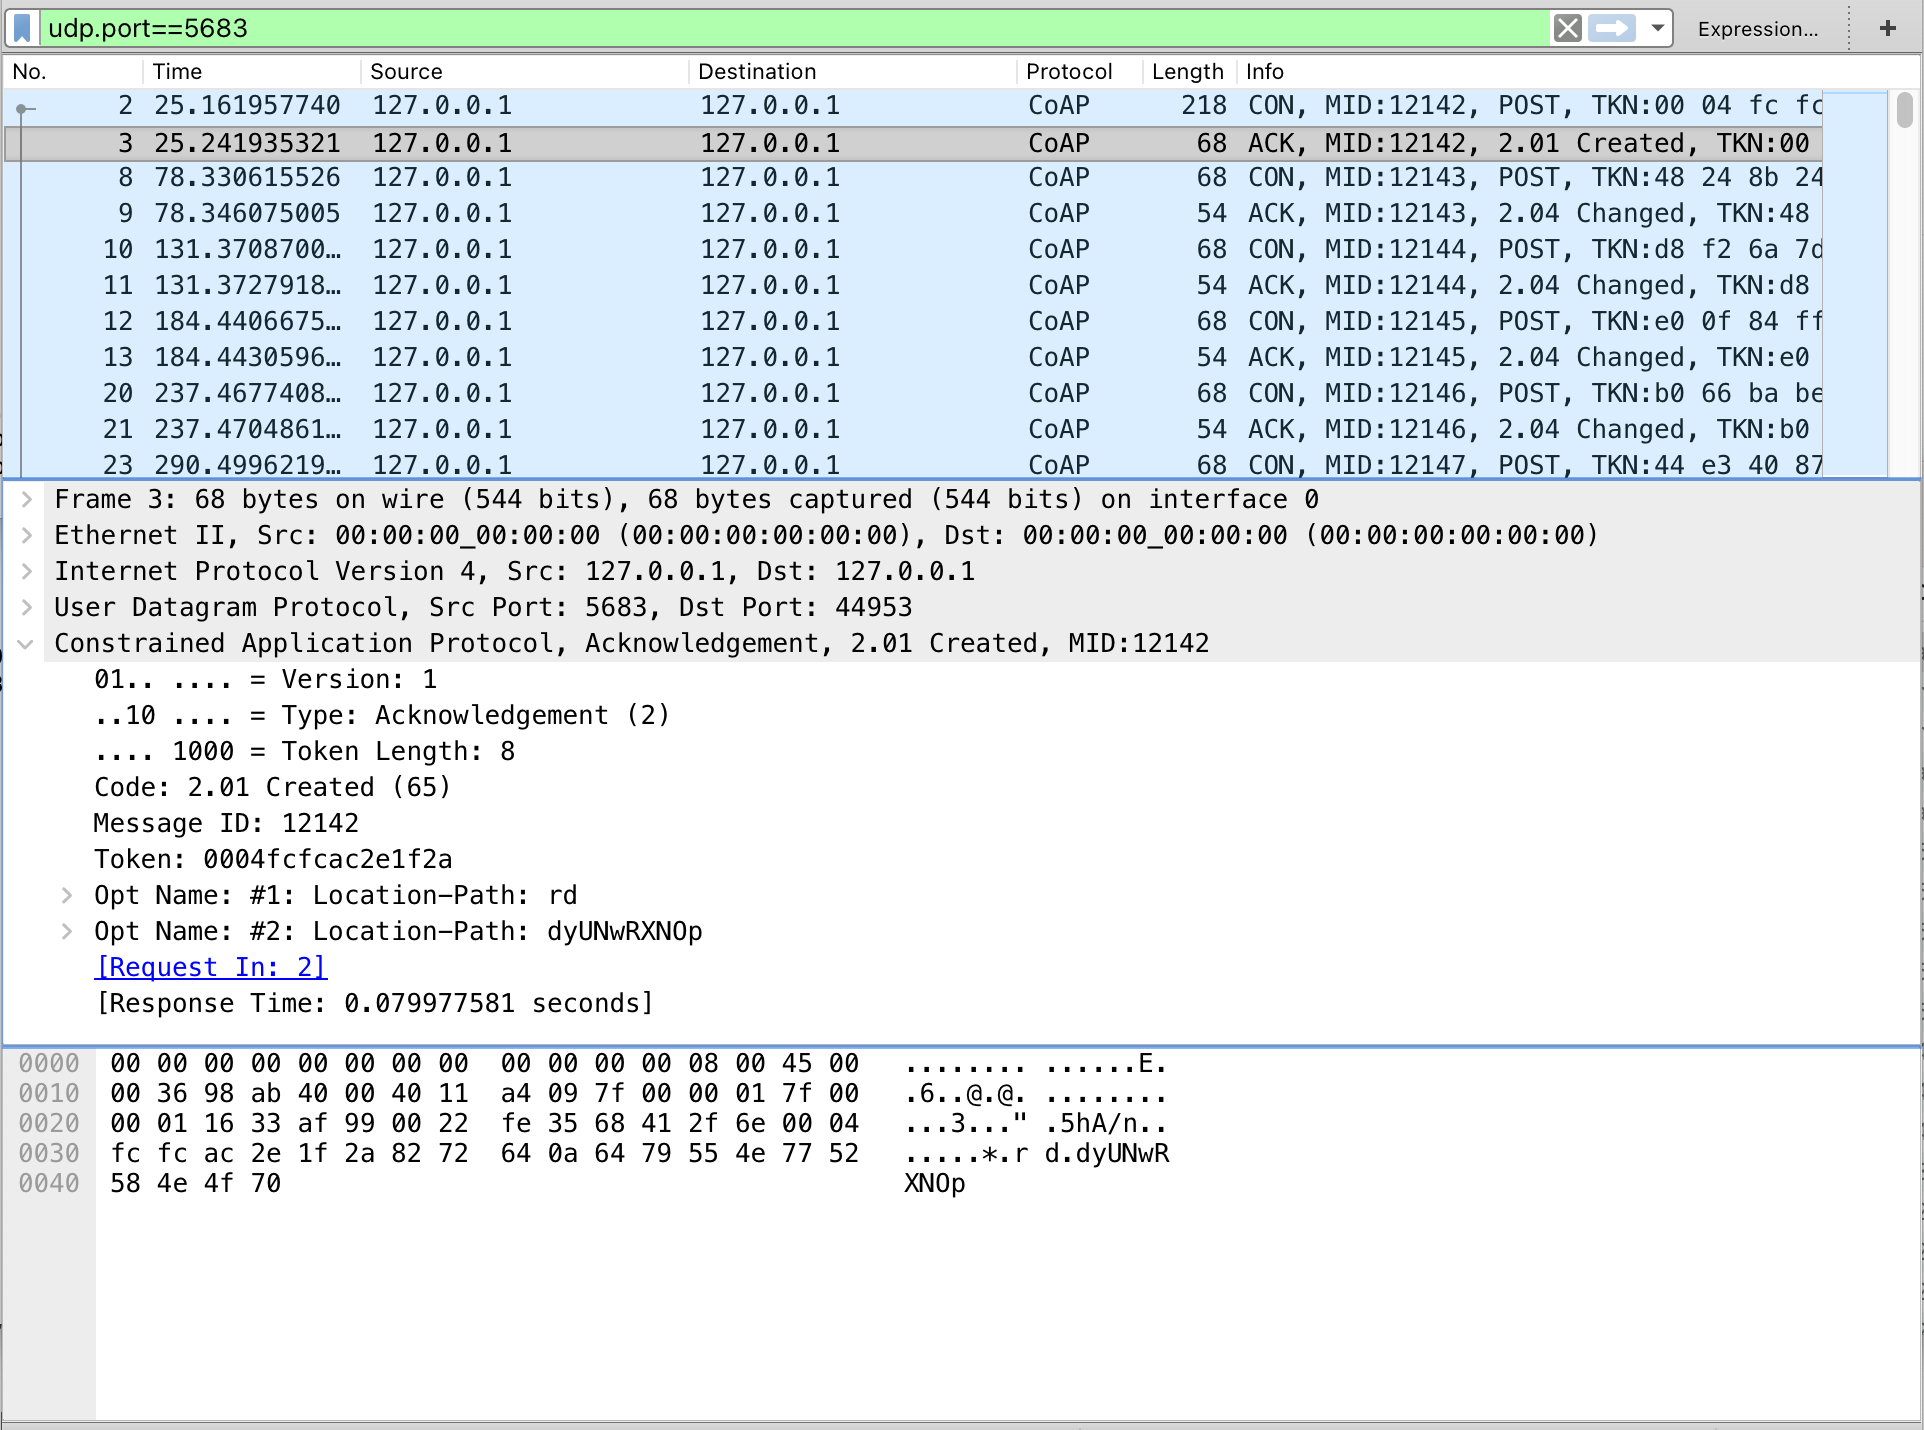
\includegraphics[width=.8\columnwidth]{Pictures/lwm2m-rep.png}}
\lgf{\caption{Réponse du serveur LwM2M au POST du client}}
\lge{\caption{LwM2M server response to client POST}}
\label{fig-lwm2m-rep}
\end{figure}

\Question{
\lgf{Réponse du serveur LwM2M}
\lge{LwM2M server response}
}
{
\lgf{Que répond le serveur (cf. figure~\vref{fig-lwm2m-rep})?}
\lge{What does the server answer (see figure~\vref{fig-lwm2m-rep})?}
\begin{itemize}[label=$\circ$]
   \item \Wrong{
    \lgf{Il acquitte juste le message.}
    \lge{It just acknowledges the message.}
    }
   \item \Wrong{
    \lgf{Rien.}
    \lgf{Nothing.}
    }
   \item \Correct{
    \lgf{Il renvoie une URI qui servira par la suite à identifier l'objet.}
    \lgf{It returns a URI that will be used later to identify the object.}
    }
   \item \Wrong{
    \lgf{Il retourne les données de chiffrement des messages.}
    \lgf{It returns the message encryption data.}
    }
\end{itemize}
}{
\lgf{La réponse contient l'option \textit{\Index{Location-Path}} ce qui permet de préciser où la ressource fournie par la client a été référencée sur le serveur. Comme pour \textit{\Index{URI-Path}}, il s'agit d'une option qui peut se répéter. Dans l'exemple,  figure~\vref{fig-lwm2m-rep}, l'URI fournie est donc \texttt{/rd/dyUNwRXNOp}.}
\lge{The response contains the option \textit{\Index{Location-Path}} which makes it possible to specify where the resource provided by the client was referenced on the server. As for \textit{\Index{URI-Path}}, it is an option which can be repeated. In the example, figure~\vref{fig-lwm2m-rep}, the URI provided is therefore \texttt{/rd/dyUNwRXNOp}.}


\lgf{Cette URI servira par la suite d'identifiant interne pour le client.}
\lge{This URI will then be used as an internal identifier for the client.}

}
 
 \Question{Wait and See}
 {
 \lgf{Si on laisse la plate-forme fonctionner sans intervenir, que voit-on sur l'analyseur réseau ?}
 \lge{If we let the platform run without intervention, what do we see on the network analyzer?}
 
 \begin{itemize}[label=$\circ$]
   \item \Wrong{
    \lgf{Rien.}
    \lge{Nothing.}
    }
   \item \Wrong{
    \lgf{Le capteur envoie des informations indiquant un changement de valeur mesurée.}
    \lge{The sensor sends information indicating a change in the measured value.}
    }
   \item \Wrong{
    \lgf{Le client envoie les valeurs mesurées même s'il elles n'ont pas changé.}
    \lge{The customer sends the measured values even if they have not changed.}
    }
   \item \Correct{
    \lgf{Le client envoie un message vide vers le serveur pour indiquer qu'il est toujours présent.}
    \lge{The client sends an empty message to the server to indicate that it is still present.}
   }
   \item \Wrong{ 
    \lgf{Le serveur envoie un message vide vers ses clients pour savoir s'ils sont toujours présents.}
    \lge{The server sends an empty message to its clients to see if they are still present.}
    }
\end{itemize}
}{
\lgf{Toutes les 53 secondes, le client envoie un POST vers la ressource créée à l'enregistrement. Ce POST est vide. Il sert à indiquer au serveur que le serveur est toujours présent. Le serveur acquitte ce message indiquant au client qu'il est aussi accessible.}
\lge{Every 53 seconds, the client sends a POST to the resource created at registration. This POST is empty. It is used to tell the server that the server is still present. The server acknowledges this message indicating to the client that it is also accessible.}

}
  
\lgf{\section{interrogation du client LwM2M}}
\lge{\section{interrogation of the LwM2M client}}

\lgf{Il est temps de revenir à l'interface de la plate-forme en ouvrant la page \texttt{http://127.0.0.1:8080} depuis le navigateur. Assurez vous que Wireshark capture toujours le trafic sur l'interface \textit{loopback}.  L'objet que nous avons inscrit apparaît. Cliquez dessus. Vous devez avoir quelque chose comme ce qui est représenté figure~\vref{fig-lwm2m-obs}.}
\lge{It is time to return to the platform interface by opening the \texttt{http://127.0.0.1:8080} page from the browser. Make sure Wireshark is still capturing traffic on the \textit{loopback} interface.  The object we have listed appears. Click on it. You should have something like what is shown in figure~\vref{fig-lwm2m-obs}.}



\begin{figure}[tbp]
\centerline{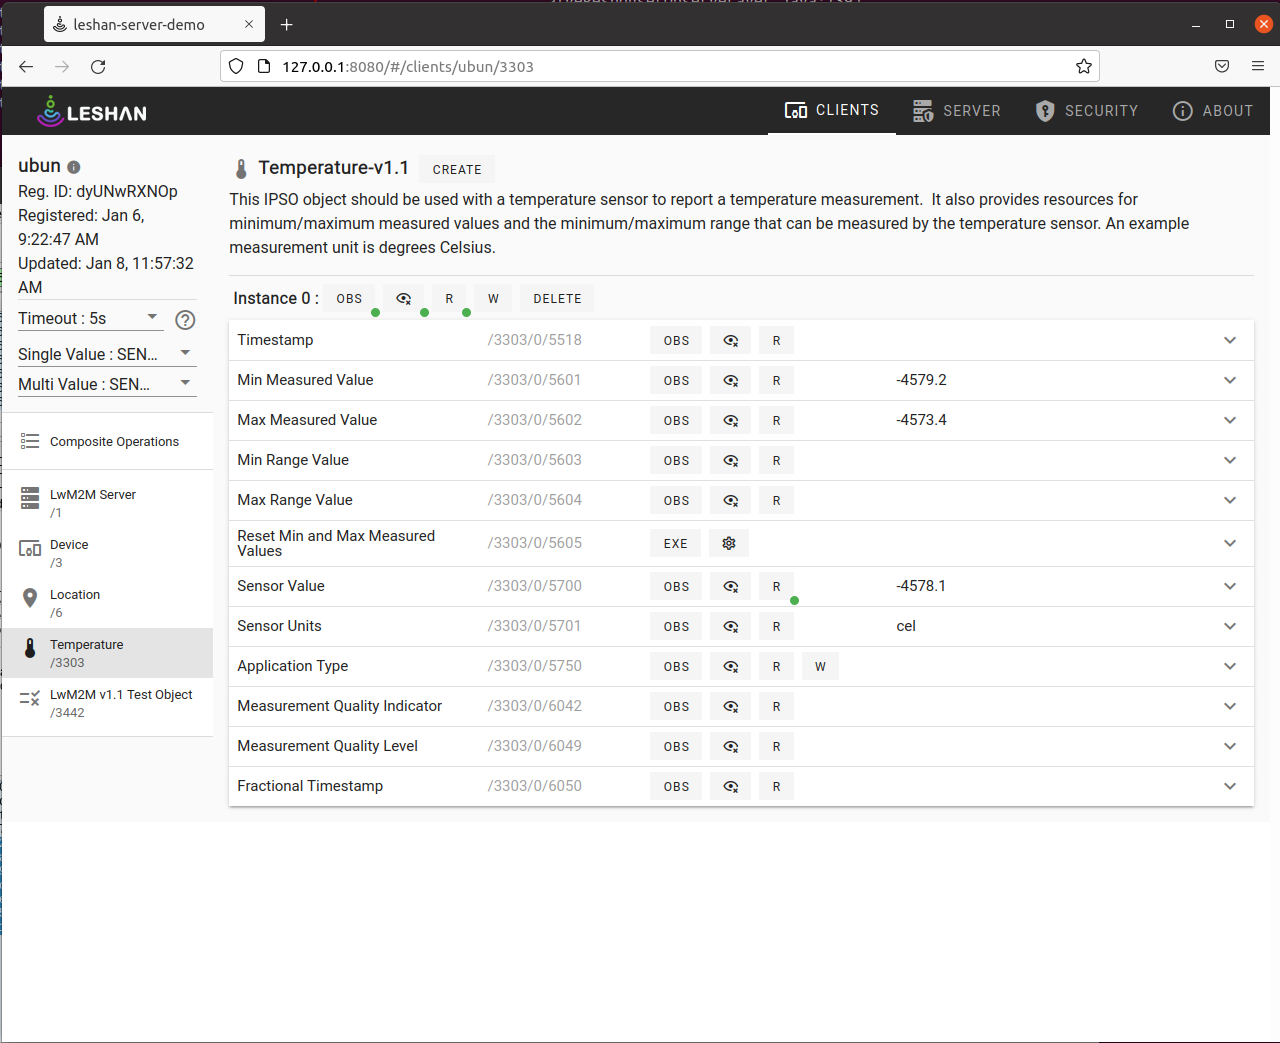
\includegraphics[width=1\columnwidth]{Pictures/lwm2m-obsever.png}}
\lgf{\caption{Visualisation du serveur LwM2M}}
\lge{\caption{Visualization of the LwM2M server}}

\label{fig-lwm2m-obs}
\end{figure}

         \vspace{1em}

\lgf{Dans le menu de gauche, on retrouve les objets numérique LwM2M décrit lors du premier POST de l'Objet.}
\lge{In the left menu, we find the LwM2M digital objects described in the first POST of the Object.}


         \vspace{1em}

\lgf{En cliquant sur \textit{Temperature}, les ressource LwM2M sont affichées. Les petits logos permettent d'effectuer des actions~:}
\lge{By clicking on \textit{Temperature}, the LwM2M resources are displayed. The small logos allow to perform actions:}

\begin{itemize}
    \item \texttt{\textit{R}} 
        \lgf{pour lire une ressource, \texttt{\textit{W}} pour l'écrire et \texttt{\textit{EXE}} pour exécuter un code (l'engrenage permet de définir les paramètres)~;}
        \lge{to read a resource, \texttt{\textit{W}} to write it and \texttt{\textit{EXE}} to execute a code (the gear allows to define the parameters);}
        
    \item \texttt{\textit{OBS}} 
        \lgf{permet de lancer un \Index{Observe} sur une ressource, L'oeil avec la croix permet d'annuler un Observe.}
        \lge{allows to launch an \Index{Observe} on a resource, the eye with the cross allows to cancel an Observe.}
\end{itemize}

\lgf{Ces actions peuvent s'appliquer individuellement à chaque ressource, ou plus globalement à une instance d'un objet numérique.}
\lge{These actions can be applied individually to each resource, or more globally to an instance of a digital object.}


\lgf{\subsection{Lecture simple}}
\lge{\subsection{Simple reading}}


\lgf{Dans le menu du gauche, sélectionnez \texit{SENML\_JSON} dans le menu déroulant \textit{Single Value}. Cela permettra d'utiliser le format \Index{SenML} plutôt que celui spécifié par LwM2M basé sur des \ac{TLV}. }
\lge{In the left-hand menu, select \texit{SENML} from the \textit{Single Value} drop-down menu. This will use the \Index{SenML} format rather than the one specified by LwM2M based on \ac{TLV}. }


         \vspace{1em}

\lgf{Pour l'objet numérique \textit{Temperature} cliquez sur le bouton \texttt{\textit{R}} de \textit{Sensor Value}. La figure~\vref{fig-lwm2m-get-simple} monte cet échange et détaille la réponse.
Le Serveur LwM2M agit comme un client REST et envoie au serveur REST du client LwM2M la requête~:}
\lge{For the numerical object \textit{Temperature} click on the button \texttt{textit{R}} of \textit{Sensor Value}. Figure~\vref{fig-lwm2m-get-simple} mounts this exchange and details the response.
The LwM2M Server acts as a REST client and sends the LwM2M client's REST server the request:}

\begin{figure}[tbp]
\centerline{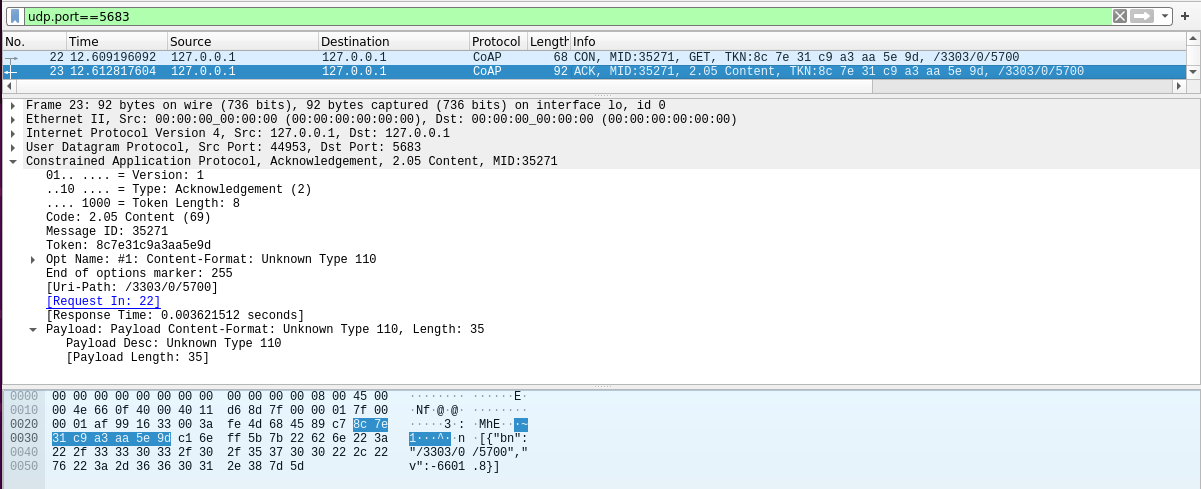
\includegraphics[width=1\columnwidth]{Pictures/lwm2m-get-simple.png}}
\lgf{\caption{Interrogation d'une ressource}}
\lge{\caption{Query a resource}}
\label{fig-lwm2m-get-simple}
\end{figure}

\begin{termc}[backgroundcolor=\color{orange!40}, basicstyle=\ttfamily\small, escapechar=@] % server
GET /3303/0/5700 
\end{termc}

\noindent 
\lgf{en indiquant le type \texttt{110} dans l'option \Index{Accept} (cf. tableau~\vref{tab-CoAP-MIME}) qui correspond au format \Index{SenML} codé en JSON . }
\lge{by indicating the type \texttt{110} in the \Index{Accept} option (cf. table~\vref{tab-CoAP-MIME}) which corresponds to the \Index{SenML} format encoded in JSON . }
    
         \vspace{1em}

\lgf{La réponse doublement associée par le même \Index{Token} et un message de type \Index{ACK} de format SenML en JSON~:  }
\lge{The response doubly associated by the same \Index{Token} and a message of type \Index{ACK} of format SenML in JSON:}



\begin{termc}[backgroundcolor=\color{purple!30}, basicstyle=\ttfamily\small, escapechar=@] % client
[{"bn":"/3303/0/5700","v":-6601.8}]
\end{termc}

\lgf{On y retrouve le nom de base (\texttt{\Index{bn}}) correspondant au nom de la ressource et la valeur (\texttt{\Index{v}})\footnote{Il est évident que le résultat retourné n'a aucun sens physique, le client LwM2M émulant mal l'évolution d'une température sur le long terme.}.}
\lge{We find the basic name (\texttt{\Index{bn}}) corresponding to the name of the resource and the value (\texttt{\Index{v}})\footnote{It is obvious that the returned result does not make any physical sense, the LwM2M client emulating poorly the evolution of a temperature on the long term}.}


          \vspace{1em}

\lgf{Cette valeur s'affiche dans la page web du serveur LwM2M, le petit point vert indiquant que l'échange s'est déroulé correctement (cf. figure~\vref{fig-lwm2m-temp-simple}).}
\lge{This value is displayed in the LwM2M server's web page, with the small green dot indicating that the exchange was successful (see figure~\vref{fig-lwm2m-temp-simple}).}


\begin{figure}[tbp]
\centerline{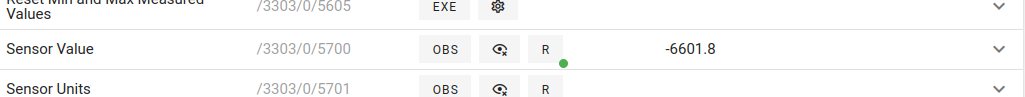
\includegraphics[width=1\columnwidth]{Pictures/lwm2m-temp-simple.png}}
\lgf{\caption{Relevé de la température}}
\lge{\caption{Temperature reading}}
\label{fig-lwm2m-temp-simple}
\end{figure}

\lgf{\subsection{Lecture d'une instance}}
\lge{\subsection{Reading an instance}}

\lgf{En  sélectionnant \texit{SENML\_JSON} dans le menu déroulant \textit{Multi Value} et en cliquant sur le bouton \texttt{\textit{R}} à droite de \textit{\textbf{Instance 0}}, différents champs de l'instance se remplissent. }
\lge{By selecting \texit{SENML\_JSON} from the \textit{Multi Value} drop-down menu and clicking on the \texttt{\textit{R}} button to the right of \textit{\textbf{Instance 0}}, various fields of the instance will be filled in. }

\lgf{L'échange protocolaire est similaire à précédent. Le serveur LwM2M a émis la requête suivante, où la valeur de la ressource est omis~:}
\lge{The protocol exchange is similar to the previous one. The LwM2M server issued the following request, where the resource value is omitted~:}


\begin{termc}[backgroundcolor=\color{orange!40}, basicstyle=\ttfamily\small, escapechar=@] % server
GET /3303/0
\end{termc}

\noindent 
\lgf{et la réponse contient~:}
\lge{and the answer contains~:}


\begin{termc}[backgroundcolor=\color{purple!30}, basicstyle=\ttfamily\small, escapechar=@] % client
[{"bn":"/3303/0/","n":"5601","v":-6672.6},
{"n":"5602","v":-4573.4},
{"n":"5700","v":-6671.6},
{"n":"5701","vs":"cel"}]
\end{termc}

\lgf{On remarque que le nom de base  (\texttt{\Index{bn}})correspond à l'URI de l'instance et que chaque éléments contient un champs nom  (\texttt{\Index{n}}) contient l'identifiant numérique de la ressource\footnote{Le champ  (\texttt{\Index{vs}}) indique que le contenu doit être interprété comme une chaîne de caractères}.}
\lge{We notice that the base name (\texttt{\Index{bn}})corresponds to the URI of the instance and that each element contains a name field (\texttt{\Index{n}}) containing the numerical identifier of the resource\footnote{The field (\texttt{\Index{vs}}) indicates that the content must be interpreted as a character string.}.}


\subsection{Observe}

\lgf{Il est aussi possible de suivre dans le temps l'état d'une ressource, nous allons le faire pour la ressource \textit{Sensor Value} de l'objet numérique \textit{Temperature}. Cliquez sur le bouton \texttt{\textit{OBS}}.}
\lge{It is also possible to follow the state of a resource over time. We will do this for the resource \textit{Sensor Value} of the digital object \textit{Temperature}. Click on the button \texttt{\textit{OBS}}.}


\lgf{Le serveur LwM2M émet la requête GET comme précédemment, en ayant inséré la l'option \textit{\Index{Observe}} avec la valeur 0 pour indiquer qu'il souhaite recevoir périodiquement des informations. Les réponses incluent également une option \textit{\Index{Observe}}  dont la valeur est croissante.}
\lge{The LwM2M server sends the GET request as before, having inserted the option \textit{\Index{Observe}} with the value 0 to indicate that it wishes to receive information periodically. The responses also include a \textit{\Index{Observe}} option with an increasing value.}


\lgf{Sur Wireshark, vous pourrez vérifier que périodiquement la réponse est envoyée en utilisant un message de type \textit{\Index{CON}firmable} plutôt que \textit{\Index{NON} confirmable} pour vérifier que le client REST sur le serveur LwM2M est toujours actif (cf figure~\vref{fig-lwm2m-obs-con})}
\lge{On Wireshark, you will be able to verify that periodically the response is sent by using a message of type \textit{\Index{CON}firmable} rather than \textit{\Index{NON} confirmable} to check that the REST client on the LwM2M server is still active (see figure~\vref{fig-lwm2m-obs-con})}


\begin{figure}[tbp]
\centerline{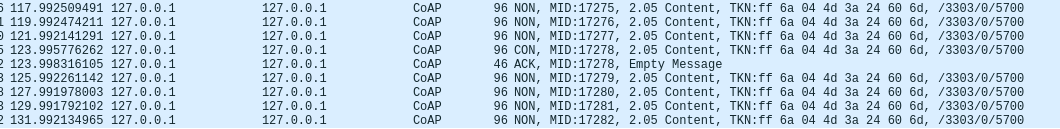
\includegraphics[width=1\columnwidth]{Pictures/lwm2m-observe-con.png}}
\lgf{\caption{Emission d'un Observe avec un message CONfirmable}}
\lgf{\caption{Sending an Observe with a CONfirmable message}}
\label{fig-lwm2m-obs-con}
\end{figure}

\Question{\lgf{Fin d'observe}\lge{End of observe}}
{
\lgf{Un click sur l'oeil avec la croix permet au serveur d'annuler l'Observe. Quel message est émis ?}
\lge{A click on the eye with the cross allows the server to cancel the Observe. What message is sent?}
}
{
\lgf{Quand le serveur LwM2M reçoit un Observe pour une session qui a été annulée, il répond avec un message de type \textit{ReSeT}, la valeur du champ \textit{Message ID} permet au client LwM2M de savoir quelle session d'Observe annuler.}
\lge{When the LwM2M server receives an Observe for a session that has been cancelled, it responds with a message of type \textit{ReSeT}, the value of the \textit{Message ID} field lets the LwM2M client know which Observe session to cancel.}
}

\Question{EXE}
{
\lgf{Quel message est émis, si on clique sur une ressource de type EXE, comme la remise à zéro des valeurs min et max?}
\lge{What message is emitted, if an EXE resource is clicked, as resetting the min and max values?}
}
{
\lgf{Cela ne change rien au protocole, un POST sur l'URI de la ressource est émis par le serveur LwM2M.}
\lge{This does not change the protocol, a POST on the URI of the resource is issued by the LwM2M server.}
}